\documentclass{standalone}

\ifstandalone
	\usepackage{amsmath}
	\usepackage{pgfplots}
\fi


\begin{document}
	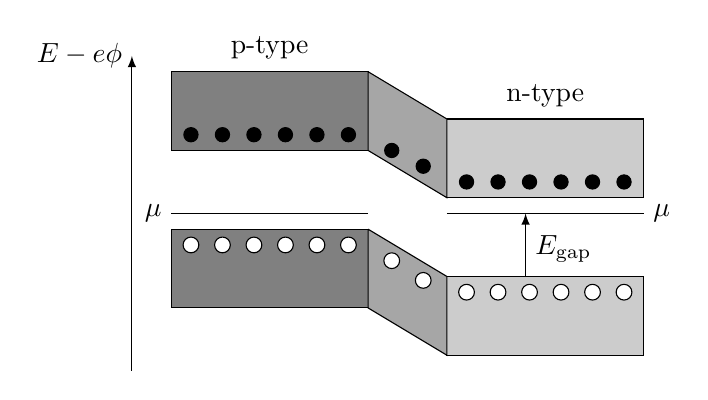
\begin{tikzpicture}
		\draw (1.25, 3.6) node {p-type};
		\draw (4.75, 3.0) node {n-type};
		\draw[-latex] (-0.5, -0.5) -- (-0.5, 3.5) node[left]{$E-e\phi$};
		\filldraw[draw=black, fill=gray] (0, 3.3) rectangle +(2.5, -1) +(0, -1.8) node[left]{$\mu$} -- +(2.5, -1.8) ++(0, -2) rectangle +(2.5, -1);
		\filldraw[draw=black, fill=gray!40] (3.5, 2.7) rectangle +(2.5, -1) +(0, -1.2) -- +(2.5, -1.2) node[right]{$\mu$} ++(0, -2) rectangle +(2.5, -1);
		\filldraw[draw=black, fill=gray!70] (2.5, 3.3) -- ++(1, -.6) -- ++(0, -1) -- ++(-1, .6) -- ++(0, 1);
		\filldraw[draw=black, fill=gray!70] (2.5, 1.3) -- ++(1, -.6) -- ++(0, -1) -- ++(-1, .6) -- ++(0, 1);
		\draw[-latex] (4.5, 0.7) -- ++(0, 0.8);
		\draw (4.5, 1.05) node[right]{$E_\text{gap}$};
		\foreach \x in {0, ..., 5} {
			\filldraw[fill=white] (0.25+0.4*\x, 1.1) circle (.10);
			\filldraw[fill=white] (3.75+0.4*\x, 0.5) circle (.10);
			\filldraw[fill=black] (3.75+0.4*\x, 1.9) circle (.09);
			\filldraw[fill=black] (0.25+0.4*\x, 2.5) circle (.09);
		};
		\filldraw[fill=white] (2.8, 0.9) circle (.10);
		\filldraw[fill=white] (3.2, 0.65) circle (.10);
		\filldraw[fill=black] (2.8, 2.3) circle (.09);
		\filldraw[fill=black] (3.2, 2.1) circle (.09);
	\end{tikzpicture}
\end{document}
